\section{Methodology}
\label{sec:workflow}
\subsection{Preliminaries}

\paragraph{Multi-turn Agent Interaction.}
% We consider a multi-turn agent interacting with an external environment over a sequence of action steps. 
We consider an agent that interacts with an external environment over multiple turns.
%
At turn $t$, the agent receives an observation $o_t$ from the environment and conditions on the full interaction history
\begin{equation}
    h_t = (o_0, a_0, o_1, a_1, \ldots, o_{t-1}, a_{t-1}, o_t),
\end{equation}
where $a_i$ denotes the model response at turn $i$. 
%
The response $a_t$ may include natural language reasoning, tool-use arguments, and an executable action. 
%
After the executable part of $a_t$ is submitted to the environment, the environment returns the next observation:
\begin{equation}
    o_{t+1} \sim \mathcal{E}(o_{t+1} \mid h_t, a_t).
\end{equation}

A complete trajectory containing $T$ turns is therefore
\begin{equation}
    \tau = (h_0, a_0, h_1, a_1, \ldots, h_{T-1}, a_{T-1}),
\end{equation}
which terminates either when a termination action is taken or when the maximum horizon $T$ is reached. 
%
This dependency distinguishes multi-turn agent learning from single-turn generation: an early mistake can alter the environment state and affect all subsequent observations.
%


\paragraph{Multi-turn On-Policy Distillation.}
Let $\pi_\theta$ denote the student policy and $\pi_\phi$ denote the teacher policy. 
%
In multi-turn OPD, trajectories are sampled from the student policy rather than from the teacher, i.e.,
\begin{equation}
    a_t \sim \pi_\theta(\cdot \mid h_t), \quad t = 0,\ldots,T-1.
\end{equation}
%
The teacher then provides supervision on the student-induced states. A standard multi-turn OPD objective applies KL-style policy distillation across the student trajectory:
\begin{equation}
    \mathcal{L}_{\mathrm{OPD}}(\theta)
    =
    \mathbb{E}_{\tau \sim \pi_\theta}
    \left[
    \sum_{t=0}^{T-1}
    D_{\mathrm{KL}}
    \left(
    \pi_\theta(\cdot \mid h_t)
    \;\middle\|\;
    \pi_\phi(\cdot \mid h_t)
    \right)
    \right],
    \label{eq:opd_loss}
\end{equation}
%
The student is trained on its own state distribution, allowing the teacher to provide feedback on states that arise from the student's behavior instead of the teacher-generated trajectories.
%

However, applying OPD uniformly to every turn in a multi-turn trajectory can be suboptimal.
%
Early student errors may alter future observations and push later histories away from the teacher's reliable state distribution, making subsequent supervision less dependable.
%
Meanwhile, token-level OPD can be brittle when teacher and student policies assign probability mass to different but semantically valid continuations, or when dense alignment reinforces local degeneracies such as repeated thoughts or actions.
%
These issues motivate a selective mechanism that decides when teacher distillation should be applied and how strongly the resulting signal should be trusted.
%


\subsection{\ours}
\label{sec:method}
\begin{figure*}[t]
    \centering
    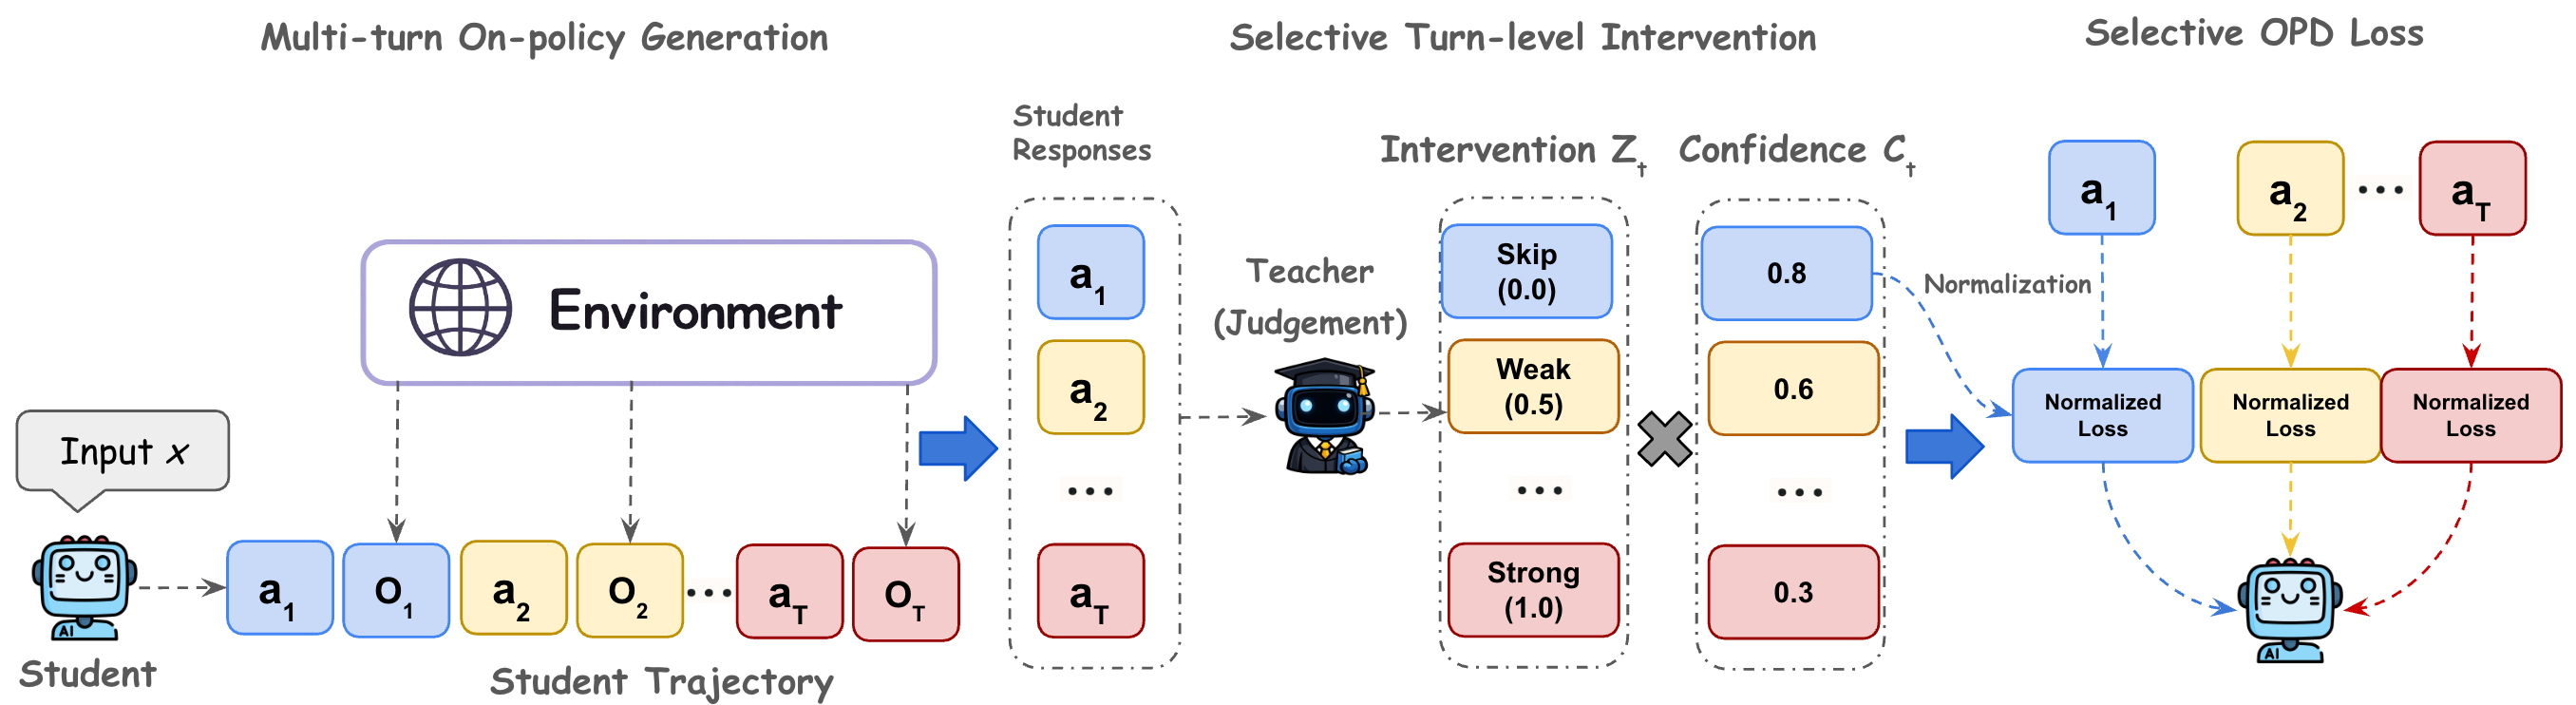
\includegraphics[width=\textwidth]{figure/diagram.png}
    \caption{
    Overview of \ours.
    %
    The student first performs multi-turn on-policy generation by interacting with the environment, producing a trajectory segmented into alternating actions and observations.
    %
    For each student turn, \ours{} uses environment feedback and teacher judgment to determine whether the response should be skipped or intervened on, and combines this intervention decision with the teacher confidence score.
    %
    The resulting selective weight modulates the OPD loss for each turn, so teacher supervision is applied more strongly when intervention is needed and the teacher signal is reliable.
    % \zz{
    % Two small comments. 
    % (1). For the annotation text of the vertical dash box containing all the actions, will ``Actions'' or ``Student Responses'' be better than ``Turn''?
    % (2). I think the diagram missed the normalization part, I understand that it is nothing too significant, but considering we've mentioned it every time when we introduce \ours, maybe it is better to add ``Vanilla-scale normalization'' below the right-most blue arrow and then make the text from ``OPD Loss'' to ``Normalized OPD Loss''?  
    % }
    }
    \label{fig:our_framework}
\end{figure*}
%
The limitations of dense multi-turn OPD suggest that teacher supervision should be applied selectively rather than uniformly across all turns.
%
Standard OPD treats a student trajectory as a flat sequence of tokens and applies teacher distillation everywhere, which makes training sensitive to token-level mismatch even when the student response is semantically acceptable.
%
Multi-turn interaction provides a natural way to move beyond this flat token-level view: the trajectory is already segmented by environment feedback, where each turn produces a response $a_t$, receives an observation, and transitions to a new history $h_{t+1}$.
%
This turn structure allows the teacher to critique larger units of behavior and decide whether token-level distillation is needed for the current student response.
%
At the same time, teacher supervision should not be trusted uniformly across the trajectory.
%
Because student errors can compound over multiple turns, later histories may drift away from the teacher's reliable state distribution, making token-level supervision less dependable.
%

Motivated by these observations, and illustrated in \figref{fig:our_framework}, we propose \ours, a selective intervention framework for multi-turn OPD.
%
For each turn, \ours{} observes the environment feedback and uses teacher judgment to decide whether the current student response should be skipped or intervened on.
%
It then weighs the token-level OPD objective by the teacher's predictive confidence, so the supervision is the strongest when intervention is needed and the teacher signal is reliable.
%
Finally, \ours{} applies loss normalization to preserve the overall loss scale of standard OPD while retaining selective turn-level weighting.
%
The full training procedure is presented in Algorithm~\ref{alg:sl_opd} in \appref{sec:implementation_details}.
%


\subsection{Turn-Level Intervention}
\label{sec:method_intervention}
To obtain turn-level supervision without a task verifier, we introduce a discrete intervention variable
\begin{equation}
    z_t \in \{\textsc{Skip}, \textsc{Weak}, \textsc{Strong}\},
    \label{eq:intervention_labels}
\end{equation}
which determines how strongly teacher distillation should be applied at turn $t$. 
%
Each intervention label is mapped to a scalar intervention weight:
\begin{equation}
    i_t (h_t, a_t) =
    \begin{cases}
        0, & z_t = \textsc{Skip}, \\
        \alpha, & z_t = \textsc{Weak}, \\
        1, & z_t = \textsc{Strong},
    \end{cases}
    \label{eq:mapping}
\end{equation}
where $\alpha \in (0,1)$ controls the strength of weak intervention. 
%
The \textsc{Skip} label suppresses OPD at the current turn, \textsc{Weak} applies partial teacher supervision, and \textsc{Strong} applies full teacher supervision.
%

We assign $z_t$ through a two-stage verifier-free procedure.
%
First, we inspect the environment feedback for deterministic interaction failures. 
%
If the student response produces a clearly invalid transition, such as a failed tool call, missing executable action, or other environment-detectable execution failure, we assign
% \begin{equation}
$z_t = \textsc{Strong}$, i.e., $i_t = 1$.
% \end{equation}
These cases do not require 
% semantic 
further second-stage judgment,
% from the teacher
since the environment already indicates that the current response should be corrected.
%

For all remaining turns, where the response is executable but its quality is ambiguous, we query the teacher with a proactive intervention-evaluation prompt (see details in \appref{sec:appendix_prompts}). 
%
Given the interaction history $h_t$, the student response $a_t$, and the available environment feedback, the teacher classifies the turn into exactly one of $\{\textsc{Skip}, \textsc{Weak}, \textsc{Strong}\}$. 
%
The resulting label is then converted into the intervention weight $i_t$ using the mapping in \eqnref{eq:mapping}. 
%
Intuitively, \textsc{Skip} is used when the response is acceptable or when multiple strategies are plausible; \textsc{Weak} is used when the response may be suboptimal but the teacher is not fully certain; and \textsc{Strong} is used when the response is clearly detrimental and teacher correction is necessary. 
%
% Prompt details are provided in \appref{sec:appendix_prompts}.


\subsection{Teacher Confidence Weighting}
The intervention label determines whether teacher supervision is needed at a given turn. 
%
However, even when the teacher identifies a turn as requiring intervention, its token-level supervision may not always be equally reliable. 
%
Due to compounding errors in multi-turn interaction, the student's previous actions may induce histories that deviate from the teacher's reliable state distribution.
%
In such cases, the teacher may still recommend intervention, but its predictive distribution can be uncertain. 
%
We therefore introduce a second factor, denoted as $c_t$, to measure the teacher's confidence in the supervision it provides at turn $t$.
%

Specifically, for each token position $i$ in the student response $a_t$, let
\begin{equation}
    p^{\star}_{t,i}
    =
    \max_{\mathcal{V}}
    \pi_{\phi}(v \mid h_t, a_{t,<i})
\end{equation}
denote the teacher's top-1 probability over the vocabulary $\mathcal{V}$.
%
This value measures how decisive the teacher is about its most likely next token at position $i$. 
%
We define the turn-level teacher confidence score as the average top-1 probability across the student response for this turn, i.e.,
\begin{equation}
    c_t(h_t,a_t)
    =
    \frac{1}{|a_t|}
    \sum_{i=1}^{|a_t|}
    p^{\star}_{t,i}
    \in (0,1].
\end{equation}
%
A sharp teacher distribution yields a high $c_t$, indicating that the teacher is confident about the token-level supervision for this turn. 
%
Conversely, a flat distribution yields a low $c_t$, indicating that the teacher itself is uncertain and that the resulting distillation signal should be weakened. 
%
This confidence term is especially important for later or off-distribution histories, where teacher intervention may be necessary but less reliable.
%

We combine the turn-level intervention weight $i_t$ with the teacher confidence score $c_t$ to obtain the final \textit{selective OPD weight}:
\begin{equation}
    s_t = i_t \cdot c_t
    \label{eq:selective_opd_weight}
\end{equation}
%
The same weight $s_t$ is applied uniformly to all token-level OPD loss within turn $t$. 
%
Note that as $p^{\star}_{t,i}$ is obtained from the same teacher distribution used for the standard distillation loss, computing $c_t$ introduces no additional teacher forward passes beyond the intervention query described in \secref{sec:method_intervention}.
% the previous subsection.
%


\subsection{Loss Normalization}
The selective weight $s_t \in [0,1]$ controls how strongly teacher supervision is applied at each token of the student response in turn $t$. 
%
However, directly multiplying the OPD loss (\eqnref{eq:opd_loss}) by $s_t$ reduces the overall gradient magnitude relative to standard OPD. 
%
Without normalization, selective weighting changes both the relative contribution of different turns and the overall magnitude of the training objective.
%
This makes it difficult to attribute performance differences specifically to selective supervision rather than to a change in optimization scale.
%
To isolate the contribution of selective weighting, we normalize the loss scale within each batch.
%

Let $\ell_{\mathrm{OPD}}(h_t,a_t)$ denote the token-level OPD loss for turn $t$, and let $N$ denote the total number of tokens in the student response of the current turn. 
%
We define the normalized selective OPD objective as
\begin{equation}
    \mathcal{L}_{\ours}
    =
    Z
    \sum_{t=0}^{T-1}
    s_t \,
    \mathcal{L}_{\mathrm{OPD}}(h_t,a_t),
\end{equation}
where the normalization factor is
\begin{equation}
    Z
    =
    \frac{N}
    {
    \max\left(
    \sum_{t=0}^{T-1} s_t |a_t|,
    \epsilon
    \right)
    }.
\end{equation}
%
Here, $|a_t|$ is the number of student tokens in turn $t$, and $\epsilon$ is a small constant for numerical stability. 
%
This normalization keeps the average effective token weight close to one, matching the scale of standard OPD while preserving the relative turn-level weighting induced by $s_t$.
%
As a result, \ours provides a verifier-free turn-level supervision policy that selectively reallocates teacher supervision without merely reducing the overall training signal.
%
